\subsection{Especificación del Plan de Pruebas}
Se realizarán cuatro tipos de pruebas para garantizar la calidad del sistema: pruebas unitarias, pruebas de integración, pruebas de usabilidad y pruebas de accesibilidad.
A continuación, se detallará cómo se llevarán a cabo las pruebas de cada tipo y se especificarán los criterios de aceptación para cada una de ellas.

\subsubsection{Pruebas Unitarias}
Las pruebas unitarias se realizarán para comprobar que cada componente del sistema funciona correctamente de forma aislada.
Se realizarán pruebas unitarias en el subsistema \textbf{restapi}, para comprobar que las rutas de la API REST funcionan correctamente, y en el subsistema \textbf{webapp}, para comprobar que los componentes de la interfaz de usuario se renderizan correctamente.

Para ello, se utilizará el framework de pruebas Jest para ambos subsistemas y se ejecutarán las pruebas en un entorno de test local.
Se espera que todas las pruebas unitarias pasen con éxito y que se alcance un porcentaje de cobertura de código mínima del 60\% para el subsistema \textbf{restapi} 
y para el subsistema \textbf{webapp} se deberán de cubrir los componentes que más se reutilizan en la aplicación.


Estas pruebas se realizarán en un entorno de test local, se utilizarán datos de prueba que simulan la información que se almacenará en la base de datos junto con una base de datos de pruebas.


\subsubsection{Pruebas de Integración}
Las pruebas de integración, también conocidas como pruebas de extremo a extremo o \textit{end-to-end}, se realizarán para comprobar que los distintos componentes del sistema funcionan correctamente en conjunto.
Se realizarán en el subsistema \textbf{webapp} con el framework de pruebas jest-cucumber y Puppeteer, que permite simular la interacción de un usuario con la aplicación y son muy descriptivas al iincluir escenarios de prueba escritos en lenguaje natural.
Estas pruebas se ejecutarán en un entorno de local de desarrollo y se utilizarán datos reales de la base de datos de desarrollo.

Los criterios de aceptación para estas pruebas son que se compruebe que un usuario puede iniciar sesión en la aplicación y que se renderice correctamente la página de inicio.

\subsubsection{Pruebas de Usabilidad}
Las pruebas de usabilidad se realizarán para comprobar que la interfaz de usuario es intuitiva y fácil de usar.
Se realizarán pruebas de usabilidad en el subsistema \textbf{webapp} con usuarios reales, que evaluarán la interfaz de usuario y proporcionarán retroalimentación sobre su usabilidad.
Estas pruebas se ejecutarán en un entorno de producción y se utilizarán datos reales de la base de datos de producción.
Los criterios de aceptación para estas pruebas son que no se reporten errores graves de usabilidad y que la interfaz de usuario sea fácil de usar para los usuarios reales.

\subsubsection{Pruebas de Accesibilidad}
Las pruebas de accesibilidad se realizarán para comprobar que la aplicación es accesible para personas con discapacidades.
Se utilizará el plugin de Google Chrome 
\coloredUnderline{\href{https://chromewebstore.google.com/detail/wave-evaluation-tool/jbbplnpkjmmeebjpijfedlgcdilocofh}{WAVE Evaluation Tool}} para comprobar la accesibilidad de la aplicación,
también se utilizará Google Lighthouse para comprobar la accesibilidad de la aplicación.

En un primer lugar se realizarán las pruebas de accesibilidad en el entorno de desarrollo y posteriormente, se repetirán en el entorno de producción con los errores corregidos.

Los criterios de aceptación para estas pruebas es que no haya errores de accesibilidad en el plugin WAVE Evaluation Tool,
permitiendo solo los errores de accesibilidad relacionados con el diseño específico de la aplicación.


\subsubsection{Pruebas de adaptabilidad}
Las pruebas de adaptabilidad se realizarán para comprobar que la aplicación se renderiza correctamente en distintos dispositivos y navegadores.
Las pruebas se realizarán en el entorno de producción y se utilizarán distintos dispositivos y navegadores para comprobar la adaptabilidad de la aplicación.
Los criterios de aceptación para estas pruebas son que la aplicación se renderice correctamente en dispositivos móviles, tabletas y ordenadores, y que funcione correctamente en los navegadores Google Chrome, Mozilla Firefox y Safari.


\subsection{Resultados de las Pruebas}
En esta sección se especificará en primer lugar las características del dispositivo y de los navegadores utilizados, y a continuación se detallarán los resultados de las pruebas realizadas.

\subsubsection{Dispositivo y navegadores utilizados}
Las pruebas se han llevado a cabo en un ordenador portátil con las siguientes características:
\begin{itemize}
    \item \textbf{Sistema Operativo}: macOS Sonoma 14.5.
    \item \textbf{Procesador}: Apple M3 Pro Max.
    \item \textbf{CPU}: 14 núcleos.
    \item \textbf{GPU}: 30 núcleos.
    \item \textbf{Memoria RAM}: 36 GB.
\end{itemize}

Como navegador se ha utilizado Google Chrome principalmente, las pruebas de adaptabilidad se han realizado además en Mozilla Firefox y Safari.
Las versiones de los navegadores son las siguientes:
\begin{itemize}
    \item \textbf{Google Chrome}: Versión 126.0.6478.127 (64 bits).
    \item \textbf{Mozilla Firefox}: Versión 127.0.2 (64 bits).
    \item \textbf{Safari}: Versión 17.5 (19618.2.12.11.6)
\end{itemize}


\subsubsection{Pruebas Unitarias}
Las pruebas unitarias se han realizado con éxito, se han comprobado que los componentes del sistema funcionan correctamente de forma aislada.
Se han realizado pruebas unitarias para cada \textit{router} del subsistema \textbf{restapi} y para los componentes más importantes del subsistema \textbf{webapp}. 

\subsubsubsection{Pruebas Unitarias. Restapi}
En el subsistema \textbf{restapi} se han realizado 51 pruebas unitarias, todas ellas han pasado con éxito obteniendo un 76.78\% de cobertura de código para \textit{routers}.
Se puede ver detallado el porcentaje de cobertura de código en la \coloredUnderline{\hyperlink{fig:6_8_Cobertura-Code-Restapi}{Figura \ref*{fig:6_8_Cobertura-Code-Restapi}: \nameref*{fig:6_8_Cobertura-Code-Restapi}}}.
\begin{figure}[H]
    \hypertarget{fig:6_8_Cobertura-Code-Restapi}{}
    \centering
    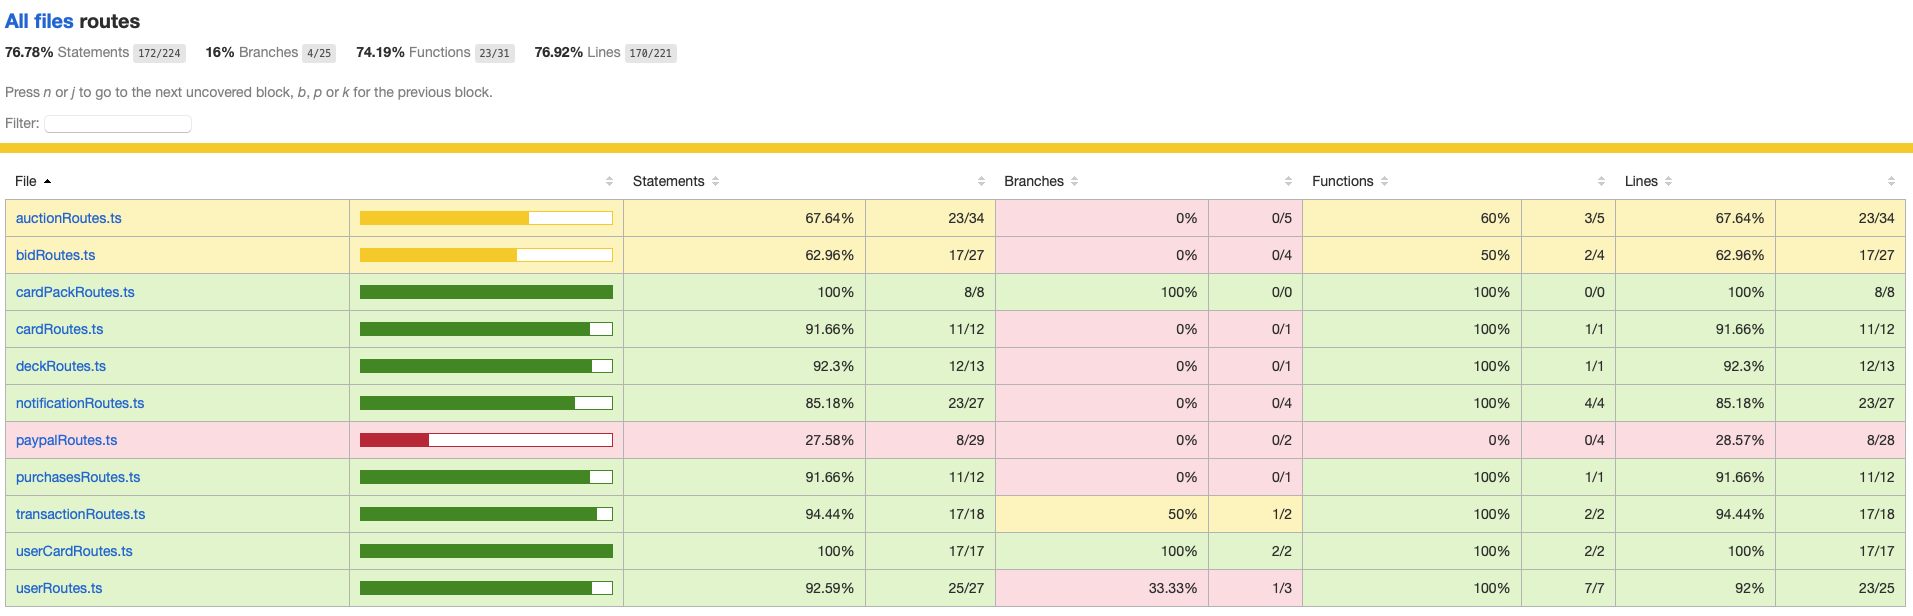
\includegraphics[width=0.8\linewidth]{figures/6-Analisis/6-Pruebas/6_8-Coverage-Restapi.png}
    \caption{Cobertura de Código del Subsistema restapi}
    \label{fig:6_8_Cobertura-Code-Restapi}
\end{figure}

A continuación, se detallan las pruebas unitarias realizadas en el subsistema \textbf{restapi}, con su descripición y resultado esperado.
Cabe destacar que para la ejecución de todas las pruebas, salvo para \textit{POST /api/users/login} y \textit{POST /api/users/signup}, se ha utilizado un token de autenticación válido, 
es decir, se ha iniciado sesión previamente con un usuario existente.


%-------------------TABLA PRUEBAS UNITARIAS RESTAPI-------------------

%-------------------TESTS DE AUCTIONROUTER-------------------
\begin{longtable}{
    >{\columncolor{lightgreen!20}}p{4cm}
    p{6cm}
    p{4cm}
    }
    \caption{Tests de auctionRouter} \label{table:test_auctionRouter} \\
    \toprule
    \rowcolor{darkgreen!50}
    \multicolumn{3}{|c|}{\textbf{Tests de auctionRouter}}\\
    \midrule
    \rowcolor{darkgreen!30}
    \textbf{Ruta a probar} & \multicolumn{1}{>{\columncolor{darkgreen!50}\centering\arraybackslash}p{6cm}}{\textbf{Descripción}} & \multicolumn{1}{>{\columncolor{darkgreen!50}\centering\arraybackslash}p{4cm}}{\textbf{Resultado esperado}} \\
    \endfirsthead
    
    \multicolumn{3}{c}%
    {{ \tablename\ \thetable{} Tests de auctionRouter -- continuación de la página anterior}} \\
    \toprule
    \rowcolor{darkgreen!50}
    \multicolumn{3}{|c|}{\textbf{Tests de auctionRouter}}\\
    \midrule
    \rowcolor{darkgreen!30}
    \textbf{Ruta a probar} & \multicolumn{1}{>{\columncolor{darkgreen!50}\centering\arraybackslash}p{6cm}}{\textbf{Descripción}} & \multicolumn{1}{>{\columncolor{darkgreen!50}\centering\arraybackslash}p{4cm}}{\textbf{Resultado esperado}} \\
    \midrule
    \endhead
    
    \midrule
    \multicolumn{3}{r}{{Continúa en la siguiente página...}} \\ 
    \endfoot
    
    \bottomrule
    \endlastfoot
    
    \midrule
    \textbf{GET /api/auctions} & Devuelve todas las subastas. & 200, la respuesta contiene una lista de subastas. \\
    \midrule
    \textbf{GET /api/auctions/a/:id} & Devuelve una subasta específica. & 200, la respuesta contiene los datos de la subasta. \\
    \midrule
    \textbf{GET /api/auctions/a/:id (no existe)} & Devuelve 404 si el ID de la subasta no se encuentra. & 404, la respuesta indica que la subasta no se encuentra. \\
    \midrule
    \textbf{GET /api/auctions/active/:username} & Devuelve todas las subastas activas para un nombre de usuario válido. & 200, la respuesta contiene una lista de subastas activas. \\
    \midrule
    \textbf{GET /api/auctions/active/u/:username} & Devuelve todas las subastas activas para un usuario. & 200, la respuesta contiene una lista de subastas activas. \\
    \end{longtable}

%-------------------TESTS DE BIDROUTER-------------------
\begin{longtable}{
    >{\columncolor{lightgreen!20}}p{4cm}
    p{6cm}
    p{4cm}
    }
    \caption{Tests de bidRouter} \label{table:test_bidRouter} \\
    \toprule
    \rowcolor{darkgreen!50}
    \multicolumn{3}{|c|}{\textbf{Tests de bidRouter}}\\
    \midrule
    \rowcolor{darkgreen!30}
    \textbf{Ruta a probar} & \multicolumn{1}{>{\columncolor{darkgreen!50}\centering\arraybackslash}p{6cm}}{\textbf{Descripción}} & \multicolumn{1}{>{\columncolor{darkgreen!50}\centering\arraybackslash}p{4cm}}{\textbf{Resultado esperado}} \\
    \endfirsthead
    
    \multicolumn{3}{c}%
    {{ \tablename\ \thetable{} Tests de bidRouter -- continuación de la página anterior}} \\
    \toprule
    \rowcolor{darkgreen!50}
    \multicolumn{3}{|c|}{\textbf{Tests de bidRouter}}\\
    \midrule
    \rowcolor{darkgreen!30}
    \textbf{Ruta a probar} & \multicolumn{1}{>{\columncolor{darkgreen!50}\centering\arraybackslash}p{6cm}}{\textbf{Descripción}} & \multicolumn{1}{>{\columncolor{darkgreen!50}\centering\arraybackslash}p{4cm}}{\textbf{Resultado esperado}} \\
    \midrule
    \endhead
    
    \midrule
    \multicolumn{3}{r}{{Continúa en la siguiente página...}} \\ 
    \endfoot
    
    \bottomrule
    \endlastfoot
    
    \midrule
    \textbf{GET /api/bids/b/:id} & Devuelve una puja específica. & 200, la respuesta contiene los datos de la puja. \\
    \midrule
    \textbf{GET /api/bids/b/:id (no existe)} & Devuelve 404 si el ID de la puja no se encuentra. & 404, la respuesta indica que la puja no se encuentra. \\
    \midrule
    \textbf{GET /api/bids/active/u/:username} & Devuelve todas las pujas activas para un nombre de usuario válido. & 200, la respuesta contiene una lista de pujas activas. \\
    \end{longtable}

%-------------------TESTS DE CARDPACKROUTER-------------------
\begin{longtable}{
    >{\columncolor{lightgreen!20}}p{4cm}
    p{6cm}
    p{4cm}
    }
    \caption{Tests de cardPackRouter} \label{table:test_cardPackRouter} \\
    \toprule
    \rowcolor{darkgreen!50}
    \multicolumn{3}{|c|}{\textbf{Tests de cardPackRouter}}\\
    \midrule
    \rowcolor{darkgreen!30}
    \textbf{Ruta a probar} & \multicolumn{1}{>{\columncolor{darkgreen!50}\centering\arraybackslash}p{6cm}}{\textbf{Descripción}} & \multicolumn{1}{>{\columncolor{darkgreen!50}\centering\arraybackslash}p{4cm}}{\textbf{Resultado esperado}} \\
    \endfirsthead
    
    \multicolumn{3}{c}%
    {{ \tablename\ \thetable{} Tests de cardPackRouter -- continuación de la página anterior}} \\
    \toprule
    \rowcolor{darkgreen!50}
    \multicolumn{3}{|c|}{\textbf{Tests de cardPackRouter}}\\
    \midrule
    \rowcolor{darkgreen!30}
    \textbf{Ruta a probar} & \multicolumn{1}{>{\columncolor{darkgreen!50}\centering\arraybackslash}p{6cm}}{\textbf{Descripción}} & \multicolumn{1}{>{\columncolor{darkgreen!50}\centering\arraybackslash}p{4cm}}{\textbf{Resultado esperado}} \\
    \midrule
    \endhead
    
    \midrule
    \multicolumn{3}{r}{{Continúa en la siguiente página...}} \\ 
    \endfoot
    
    \bottomrule
    \endlastfoot
    
    \midrule
    \textbf{GET /api/cardpacks} & Devuelve todos los paquetes de cartas disponibles. & 200, la respuesta contiene una lista de paquetes de cartas filtrados por disponibilidad. \\
    \end{longtable}

%-------------------TESTS DE CARDROUTER-------------------
\begin{longtable}{
    >{\columncolor{lightgreen!20}}p{4cm}
    p{6cm}
    p{4cm}
    }
    \caption{Tests de cardRouter} \label{table:test_cardRouter} \\
    \toprule
    \rowcolor{darkgreen!50}
    \multicolumn{3}{|c|}{\textbf{Tests de cardRouter}}\\
    \midrule
    \rowcolor{darkgreen!30}
    \textbf{Ruta a probar} & \multicolumn{1}{>{\columncolor{darkgreen!50}\centering\arraybackslash}p{6cm}}{\textbf{Descripción}} & \multicolumn{1}{>{\columncolor{darkgreen!50}\centering\arraybackslash}p{4cm}}{\textbf{Resultado esperado}} \\
    \endfirsthead
    
    \multicolumn{3}{c}%
    {{ \tablename\ \thetable{} Tests de cardRouter -- continuación de la página anterior}} \\
    \toprule
    \rowcolor{darkgreen!50}
    \multicolumn{3}{|c|}{\textbf{Tests de cardRouter}}\\
    \midrule
    \rowcolor{darkgreen!30}
    \textbf{Ruta a probar} & \multicolumn{1}{>{\columncolor{darkgreen!50}\centering\arraybackslash}p{6cm}}{\textbf{Descripción}} & \multicolumn{1}{>{\columncolor{darkgreen!50}\centering\arraybackslash}p{4cm}}{\textbf{Resultado esperado}} \\
    \midrule
    \endhead
    
    \midrule
    \multicolumn{3}{r}{{Continúa en la siguiente página...}} \\ 
    \endfoot
    
    \bottomrule
    \endlastfoot
    
    \midrule
    \textbf{GET /api/cards/:cardId} & Devuelve una carta por su ID. & 200, la respuesta contiene los datos de la carta, incluyendo el nombre 'bulbasaur'. \\
    \midrule
    \textbf{GET /api/cards/:cardId (no existe)} & Devuelve 404 si la carta no se encuentra. & 404, la respuesta contiene el mensaje 'Carta no encontrada.'. \\
    \midrule
    \textbf{GET /api/cards/:cardId (error)} & Maneja errores de forma adecuada. & 500, la respuesta contiene el mensaje 'Se ha producido un error al obtener la carta.'. \\
    \end{longtable}



%-------------------TESTS DE DECKROUTER-------------------

\begin{longtable}{
    >{\columncolor{lightgreen!20}}p{4cm}
    p{6cm}
    p{4cm}
    }
    \caption{Tests de deckRouter} \label{table:test_deckRouter} \\
    \toprule
    \rowcolor{darkgreen!50}
    \multicolumn{3}{|c|}{\textbf{Tests de deckRouter}}\\
    \midrule
    \rowcolor{darkgreen!30}
    \textbf{Ruta a probar} & \multicolumn{1}{>{\columncolor{darkgreen!50}\centering\arraybackslash}p{6cm}}{\textbf{Descripción}} & \multicolumn{1}{>{\columncolor{darkgreen!50}\centering\arraybackslash}p{4cm}}{\textbf{Resultado esperado}} \\
    \endfirsthead
    
    \multicolumn{3}{c}%
    {{ \tablename\ \thetable{} Tests de deckRouter -- continuación de la página anterior}} \\
    \toprule
    \rowcolor{darkgreen!50}
    \multicolumn{3}{|c|}{\textbf{Tests de deckRouter}}\\
    \midrule
    \rowcolor{darkgreen!30}
    \textbf{Ruta a probar} & \multicolumn{1}{>{\columncolor{darkgreen!50}\centering\arraybackslash}p{6cm}}{\textbf{Descripción}} & \multicolumn{1}{>{\columncolor{darkgreen!50}\centering\arraybackslash}p{4cm}}{\textbf{Resultado esperado}} \\
    \midrule
    \endhead
    
    \midrule
    \multicolumn{3}{r}{{Continúa en la siguiente página...}} \\ 
    \endfoot
    
    \bottomrule
    \endlastfoot
    
    \midrule
    \textbf{GET /api/decks} & Devuelve todos los mazos de cartas. & 200, la respuesta contiene una lista de mazos de cartas. \\
    \midrule
    \textbf{GET /api/decks/:deckid} & Devuelve un mazo de cartas por su ID. & 200, la respuesta contiene los datos del mazo de cartas, incluyendo 'deckId', 'name', 'type', y 'publicationDate'. \\
    \midrule
    \textbf{GET /api/decks (error)} & Maneja errores de forma adecuada al obtener todos los mazos de cartas. & 500, la respuesta contiene el mensaje 'Se ha producido un error al obtener los mazos de cartas.'. \\
    \midrule
    \textbf{GET /api/decks/:deckid (no existe)} & Devuelve 404 si el mazo de cartas no se encuentra. & 404, la respuesta contiene el mensaje 'Mazo de cartas no encontrado.'. \\
    \midrule
    \textbf{GET /api/decks/:deckid (error)} & Maneja errores de forma adecuada al obtener un mazo de cartas por su ID. & 500, la respuesta contiene el mensaje 'Se ha producido un error al obtener el mazo de cartas.'. \\
    \end{longtable}


%-------------------TESTS DE NOTIFICATIONROUTER-------------------
\begin{longtable}{
    >{\columncolor{lightgreen!20}}p{4cm}
    p{6cm}
    p{4cm}
    }
    \caption{Tests de notificationRouter} \label{table:test_notificationRouter} \\
    \toprule
    \rowcolor{darkgreen!50}
    \multicolumn{3}{|c|}{\textbf{Tests de notificationRouter}}\\
    \midrule
    \rowcolor{darkgreen!30}
    \textbf{Ruta a probar} & \multicolumn{1}{>{\columncolor{darkgreen!50}\centering\arraybackslash}p{6cm}}{\textbf{Descripción}} & \multicolumn{1}{>{\columncolor{darkgreen!50}\centering\arraybackslash}p{4cm}}{\textbf{Resultado esperado}} \\
    \endfirsthead
    
    \multicolumn{3}{c}%
    {{ \tablename\ \thetable{} Tests de notificationRouter -- continuación de la página anterior}} \\
    \toprule
    \rowcolor{darkgreen!50}
    \multicolumn{3}{|c|}{\textbf{Tests de notificationRouter}}\\
    \midrule
    \rowcolor{darkgreen!30}
    \textbf{Ruta a probar} & \multicolumn{1}{>{\columncolor{darkgreen!50}\centering\arraybackslash}p{6cm}}{\textbf{Descripción}} & \multicolumn{1}{>{\columncolor{darkgreen!50}\centering\arraybackslash}p{4cm}}{\textbf{Resultado esperado}} \\
    \midrule
    \endhead
    
    \midrule
    \multicolumn{3}{r}{{Continúa en la siguiente página...}} \\ 
    \endfoot
    
    \bottomrule
    \endlastfoot
    
    \midrule
    \textbf{GET /api/notifications/:username} & Devuelve todas las notificaciones para un nombre de usuario válido. & 200, la respuesta contiene una lista de notificaciones. \\
    \midrule
    \textbf{GET /api/notifications/unread/:username} & Devuelve todas las notificaciones no leídas para un nombre de usuario válido. & 200, la respuesta contiene una lista de notificaciones no leídas. \\
    \midrule
    \textbf{PATCH /api/notifications/notification/:notificationId/read} & Marca una notificación como leída. & 200, la respuesta indica éxito. \\
    \midrule
    \textbf{PATCH /api/notifications/read/:username} & Marca todas las notificaciones de un usuario como leídas. & 200, la respuesta indica éxito. \\
    \end{longtable}


%-------------------TESTS DE PURCHASESROUTER-------------------
\begin{longtable}{
    >{\columncolor{lightgreen!20}}p{4cm}
    p{6cm}
    p{4cm}
    }
    \caption{Tests de purchasesRouter} \label{table:test_purchasesRouter} \\
    \toprule
    \rowcolor{darkgreen!50}
    \multicolumn{3}{|c|}{\textbf{Tests de purchasesRouter}}\\
    \midrule
    \rowcolor{darkgreen!30}
    \textbf{Ruta a probar} & \multicolumn{1}{>{\columncolor{darkgreen!50}\centering\arraybackslash}p{6cm}}{\textbf{Descripción}} & \multicolumn{1}{>{\columncolor{darkgreen!50}\centering\arraybackslash}p{4cm}}{\textbf{Resultado esperado}} \\
    \endfirsthead
    
    \multicolumn{3}{c}%
    {{ \tablename\ \thetable{} Tests de purchasesRouter -- continuación de la página anterior}} \\
    \toprule
    \rowcolor{darkgreen!50}
    \multicolumn{3}{|c|}{\textbf{Tests de purchasesRouter}}\\
    \midrule
    \rowcolor{darkgreen!30}
    \textbf{Ruta a probar} & \multicolumn{1}{>{\columncolor{darkgreen!50}\centering\arraybackslash}p{6cm}}{\textbf{Descripción}} & \multicolumn{1}{>{\columncolor{darkgreen!50}\centering\arraybackslash}p{4cm}}{\textbf{Resultado esperado}} \\
    \midrule
    \endhead
    
    \midrule
    \multicolumn{3}{r}{{Continúa en la siguiente página...}} \\ 
    \endfoot
    
    \bottomrule
    \endlastfoot
    
    \midrule
    \textbf{POST /api/purchases/cardpack} & Compra un paquete de cartas exitosamente, disminuyendo la cantidad disponible del paquete y el saldo del usuario, creando cartas de usuario y transacciones. & 200, la respuesta indica éxito y las verificaciones post-compra son correctas. \\
    \midrule
    \textbf{POST /api/purchases/cardpack (usuario no existe)} & Maneja errores cuando el usuario no existe. & 500, la respuesta contiene el mensaje 'El usuario no existe.'. \\
    \midrule
    \textbf{POST /api/purchases/cardpack (saldo insuficiente)} & Maneja errores cuando el usuario no tiene suficiente saldo. & 500, la respuesta indica un error de saldo insuficiente. \\
    \midrule
    \textbf{POST /api/purchases/cardpack (paquete no existe)} & Maneja errores cuando el paquete de cartas no existe. & 500, la respuesta indica que el paquete de cartas no se encuentra. \\
    \midrule
    \textbf{POST /api/purchases/cardpack (paquete no disponible)} & Maneja errores cuando el paquete de cartas no está disponible. & 500, la respuesta indica que el paquete de cartas no está disponible. \\
    \end{longtable}



%-------------------TESTS DE TRANSACTIONROUTER-------------------
\begin{longtable}{
    >{\columncolor{lightgreen!20}}p{4cm}
    p{6cm}
    p{4cm}
    }
    \caption{Tests de transactionRouter} \label{table:descripcion_transactionRouter} \\
    \toprule
    \rowcolor{darkgreen!50}
    \multicolumn{3}{|c|}{\textbf{Tests de transactionRouter}}\\
    \midrule
    \rowcolor{darkgreen!30}
    \textbf{Ruta a probar} & \multicolumn{1}{>{\columncolor{darkgreen!50}\centering\arraybackslash}p{6cm}}{\textbf{Descripción}} & \multicolumn{1}{>{\columncolor{darkgreen!50}\centering\arraybackslash}p{4cm}}{\textbf{Resultado esperado}} \\
    \endfirsthead
    
    \multicolumn{3}{c}%
    {{ \tablename\ \thetable{} Tests de transactionRouter -- continuación de la página anterior}} \\
    \toprule
    \rowcolor{darkgreen!50}
    \multicolumn{3}{|c|}{\textbf{Tests de transactionRouter}}\\
    \midrule
    \rowcolor{darkgreen!30}
    \textbf{Ruta a probar} & \multicolumn{1}{>{\columncolor{darkgreen!50}\centering\arraybackslash}p{6cm}}{\textbf{Descripción}} & \multicolumn{1}{>{\columncolor{darkgreen!50}\centering\arraybackslash}p{4cm}}{\textbf{Resultado esperado}} \\
    \midrule
    \endhead
    
    \midrule
    \multicolumn{3}{r}{{Continúa en la siguiente página...}} \\ 
    \endfoot
    
    \bottomrule
    \endlastfoot
    
    \midrule
    \textbf{GET /api/transactions} & Devuelve todas las transacciones. & 200, la respuesta contiene una lista de transacciones. \\
    \midrule
    \textbf{GET /api/transactions/u/:username} & Devuelve las transacciones para un nombre de usuario válido. & 200, la respuesta contiene una lista de transacciones para el usuario. \\
    \midrule
    \textbf{GET /api/transactions/c/:userCardId} & Devuelve las transacciones para un ID de carta de usuario válido. & 200, la respuesta contiene una lista de transacciones para la carta de usuario. \\
    \midrule
    \textbf{GET /api/transactions (no admin)} & Devuelve 403 si el usuario no es administrador. & 403, la respuesta contiene el mensaje 'Acceso denegado. Se requiere rol de administrador.'. \\
    \midrule
    \textbf{GET /api/transactions/u/:username (username inválido)} & Devuelve 400 para un nombre de usuario inválido. & 400, la respuesta contiene errores de validación para el nombre de usuario. \\
    \end{longtable}



%-------------------TESTS DE USERCARDROUTER-------------------
\begin{longtable}{
    >{\columncolor{lightgreen!20}}p{4cm}
    p{6cm}
    p{4cm}
    }
    \caption{Tests de userCardRouter} \label{table:test_userCardRouter} \\
    \toprule
    \rowcolor{darkgreen!50}
    \multicolumn{3}{|c|}{\textbf{Tests de userCardRouter}}\\
    \midrule
    \rowcolor{darkgreen!30}
    \textbf{Ruta a probar} & \multicolumn{1}{>{\columncolor{darkgreen!50}\centering\arraybackslash}p{6cm}}{\textbf{Descripción}} & \multicolumn{1}{>{\columncolor{darkgreen!50}\centering\arraybackslash}p{4cm}}{\textbf{Resultado esperado}} \\
    \endfirsthead
    
    \multicolumn{3}{c}%
    {{ \tablename\ \thetable{} Tests de userCardRouter -- continuación de la página anterior}} \\
    \toprule
    \rowcolor{darkgreen!50}
    \multicolumn{3}{|c|}{\textbf{Tests de userCardRouter}}\\
    \midrule
    \rowcolor{darkgreen!30}
    \textbf{Ruta a probar} & \multicolumn{1}{>{\columncolor{darkgreen!50}\centering\arraybackslash}p{6cm}}{\textbf{Descripción}} & \multicolumn{1}{>{\columncolor{darkgreen!50}\centering\arraybackslash}p{4cm}}{\textbf{Resultado esperado}} \\
    \midrule
    \endhead
    
    \midrule
    \multicolumn{3}{r}{{Continúa en la siguiente página...}} \\ 
    \endfoot
    
    \bottomrule
    \endlastfoot
    
    \midrule
    \textbf{GET /api/usercards/u/:username} & Devuelve las tarjetas de usuario para un nombre de usuario válido. & 200, la respuesta contiene un arreglo de tarjetas de usuario. \\
    \midrule
    \textbf{GET /api/usercards/:id} & Devuelve una tarjeta de usuario específica. & 200, la respuesta contiene la tarjeta de usuario con el campo 'legibleCardId'. \\
    \midrule
    \textbf{GET /api/usercards/:id (no existe)} & Devuelve 404 si la tarjeta de usuario no se encuentra. & 404, la respuesta indica que la tarjeta de usuario no se encuentra. \\
    \midrule
    \textbf{GET /api/usercards/:id (ID inválido)} & Devuelve 400 para un ID de tarjeta de usuario inválido. & 400, la respuesta indica un error. \\
    \midrule
    \textbf{GET /api/usercards/u/:username (nombre de usuario muy largo)} & Devuelve 400 si el nombre de usuario es demasiado largo. & 400, la respuesta indica un error con un mensaje sobre la longitud del nombre de usuario. \\
    \end{longtable}

%-------------------TESTS DE USERROUTER-------------------
\begin{longtable}{
    >{\columncolor{lightgreen!20}}p{4cm}
    p{6cm}
    p{4cm}
    }
    \caption{Tests de userRouter} \label{table:test_userRouter} \\
    \toprule
    \rowcolor{darkgreen!50}
    \multicolumn{3}{|c|}{\textbf{Tests de userRouter}}\\
    \midrule
    \rowcolor{darkgreen!30}
    \textbf{Ruta a probar} & \multicolumn{1}{>{\columncolor{darkgreen!50}\centering\arraybackslash}p{6cm}}{\textbf{Descripción}} & \multicolumn{1}{>{\columncolor{darkgreen!50}\centering\arraybackslash}p{4cm}}{\textbf{Resultado esperado}} \\
    \endfirsthead
    
    \multicolumn{3}{c}%
    {{ \tablename\ \thetable{} Tests de userRouter -- continuación de la página anterior}} \\
    \toprule
    \rowcolor{darkgreen!50}
    \multicolumn{3}{|c|}{\textbf{Tests de userRouter}}\\
    \midrule
    \rowcolor{darkgreen!30}
    \textbf{Ruta a probar} & \multicolumn{1}{>{\columncolor{darkgreen!50}\centering\arraybackslash}p{6cm}}{\textbf{Descripción}} & \multicolumn{1}{>{\columncolor{darkgreen!50}\centering\arraybackslash}p{4cm}}{\textbf{Resultado esperado}} \\
    \midrule
    \endhead
    
    \midrule
    \multicolumn{3}{r}{{Continúa en la siguiente página...}} \\ 
    \endfoot
    
    \bottomrule
    \endlastfoot
    
    \midrule
    \textbf{POST /api/users/login} & Inicia sesión un usuario existente con el nombre de usuario 'test' y la contraseña 'Password123-'. & 200, la respuesta contiene un token y datos del usuario. \\
    \midrule
    \textbf{POST /api/users/signup} & Crea un nuevo usuario con el nombre de usuario 'newuser' y la contraseña 'Password123-'. & 201, la respuesta contiene un mensaje de éxito y datos del nuevo usuario. \\
    \midrule
    \textbf{GET /api/users/:username} & Obtiene los detalles del usuario 'test' con un token válido. & 200, la respuesta contiene los datos del usuario. \\
    \midrule
    \textbf{PATCH /api/users/update/avatar} & Actualiza la imagen de perfil del usuario 'test' a 'avatar1.png'. & 200, la respuesta indica éxito. \\
    \midrule
    \textbf{PATCH /api/users/update/pass} & Actualiza la contraseña del usuario 'test' a 'NewPass1234-'. & 200, la respuesta indica éxito. \\
    \midrule
    \textbf{GET /api/users/:username (error handling)} & Devuelve 400 si el nombre de usuario es demasiado largo. & 400, la respuesta indica error. \\
    \midrule
    \textbf{GET /api/users/:username (sin token)} & Devuelve 401 si no se proporciona un token. & 401, la respuesta indica error. \\
    \midrule
    \textbf{GET /api/users/:username (usuario no encontrado)} & Devuelve 404 si el usuario no se encuentra. & 404, la respuesta contiene mensaje de usuario no encontrado. \\
    \midrule
    \textbf{GET /api/users/:username (error)} & Maneja errores de forma adecuada. & 500, la respuesta indica error interno. \\
    \midrule
    \textbf{POST /api/users/login (usuario no existe)} & Devuelve 401 si el usuario no existe. & 401, la respuesta indica error. \\
    \midrule
    \textbf{POST /api/users/login (contraseña incorrecta)} & Devuelve 401 si la contraseña es incorrecta. & 401, la respuesta indica error. \\
    \midrule
    \textbf{POST /api/users/login (error)} & Maneja errores de forma adecuada. & 500, la respuesta indica error interno. \\
    \midrule
    \textbf{POST /api/users/signup (usuario ya existe)} & Devuelve 400 si el nombre de usuario ya existe. & 400, la respuesta indica error. \\
    \midrule
    \textbf{POST /api/users/signup (datos incompletos)} & Devuelve 400 si falta el nombre de usuario, contraseña o fecha de nacimiento. & 400, la respuesta indica error. \\
    \midrule
    \textbf{POST /api/users/signup (error)} & Maneja errores de forma adecuada. & 500, la respuesta contiene mensaje de error y autenticación fallida. \\
    \end{longtable}




\subsubsubsection{Pruebas Unitarias. Webapp}
En el subsistema \textbf{webapp} se han realizado 9 pruebas unitarias automáticas, se han probado los componentes más importantes de la aplicación y todas han pasado con éxito.
El resto de componentes se han probado de forma manual y se ha comprobado que su comportamiento es el esperado.
Las pruebas unitarias automáticas se han realizado sobre los componentes que más se reutilizan en la aplicación, estos son:
\begin{itemize}
    \item \textbf{Componente \textit{Button}}: Se ha comprobado que el componente \textit{Button} renderiza correctamente, que se muestra el texto esperado y que se ejecuta la función \textit{onClick} cuando se hace clic en el botón.
    \item \textbf{Componente \textit{Calendar}}: Se ha comprobado que el componente \textit{Calendar} renderiza correctamente, que se ejecuta la función \textit{onChange} cuando se selecciona una fecha y que si hay un error en la fecha se muestre un mensaje de error.
    \item \textbf{Componente \textit{ErrorMessageBox}}: Se ha comprobado que el componente \textit{ErrorMessageBox} renderiza correctamente y que redirige a la página de inicio cuando se hace clic en el botón que contiene.
    \item \textbf{Componente \textit{PokemonCard}}: Se ha comprobado que la carta de Pokémon se renderiza correctamente y que se ejecutan los distintos \textit{onClick} dependiendo de su configuración inicial.
\end{itemize}
En la figura \coloredUnderline{\hyperlink{fig:coverage_webapp}{Figura \ref*{fig:coverage_webapp}. \nameref*{fig:coverage_webapp}}} se muestran los resultados de las pruebas unitarias automáticas realizadas.
\begin{figure}[H]
    \centering
    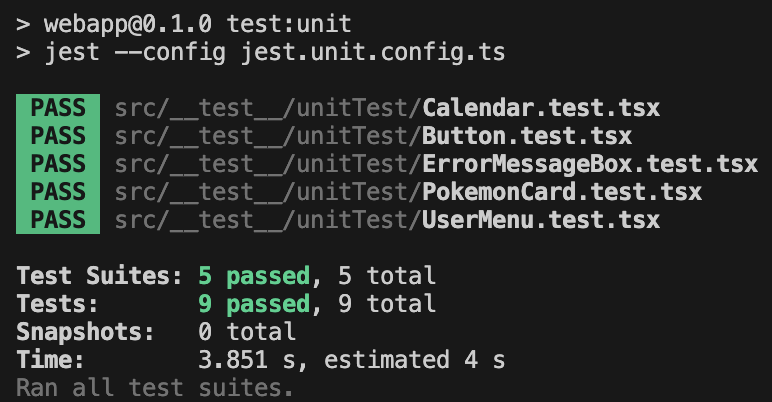
\includegraphics[width=0.5\textwidth]{figures/6-Analisis/6-Pruebas/6_8_webapp-unit.png}
    \caption{Resultados de las pruebas unitarias automáticas de la webapp}
    \hypertarget{fig:coverage_webapp}{}
    \label{fig:coverage_webapp}
\end{figure}

\subsubsection{Pruebas de Integración}
Las pruebas de integración se han realizado con éxito, se han comprobado que los distintos componentes del sistema funcionan correctamente en conjunto.
Se han realizado pruebas de integración en el subsistema \textbf{webapp} con el framework jest-cucumber y Puppeteer.
Se han realizado 3 pruebas de integración automáticas, todas ellas han pasado con éxito.
Las pruebas que se han realizado son las siguientes:
\begin{itemize}
    \item \textbf{Prueba de Inicio de Sesión Exitoso}: Se ha comprobado que el inicio de sesión funciona correctamente. De esta forma, se ha comprobado que el usuario puede iniciar sesión con sus credenciales y acceder a la aplicación, 
    lo que significa que la conexión con el backend funciona correctamente y la integración de los componentes de la aplicación es correcta.
    \item \textbf{Prueba de Inicio de Sesión Fallido}: Se ha comprobado que el inicio de sesión falla cuando las credenciales son incorrectas. De esta forma, se ha comprobado que la aplicación responde correctamente a errores en el inicio de sesión.
     \item \textbf{Prueba de Registro de Usuario Fallido}: Se ha comprobado que el registro de usuario falla cuando los datos introducidos no son válidos. 
     Se verifica que la aplicación responde correctamente a errores en el registro de usuario y se resaltan los campos con errores.
\end{itemize}

En la figura \coloredUnderline{\hyperlink{fig:coverage_webapp2}{Figura \ref*{fig:coverage_webapp}. \nameref*{fig:coverage_webapp}}} se muestran los resultados de las pruebas de integración automáticas realizadas.
\begin{figure}[H]
    \centering
    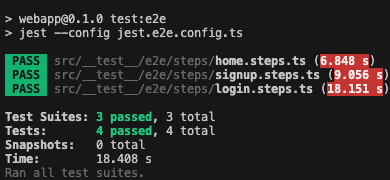
\includegraphics[width=0.5\textwidth]{figures/6-Analisis/6-Pruebas/6_8_webapp-e2e.png}
    \caption{Resultados de las pruebas de integración automáticas de la webapp}
    \hypertarget{fig:coverage_webapp2}{}
    \label{fig:coverage_webapp2}
\end{figure}

El resto de pruebas de integración se han realizado de forma manual y se ha comprobado que el comportamiento de la aplicación es el esperado.

\subsubsection{Pruebas de Usabilidad}
Se ha creado un formulario de evaluación de usabilidad que se les ha proporcionado a los usuarios para que evalúen la interfaz de usuario.
Se han realizado pruebas de usabilidad con 3 usuarios reales, que han evaluado la interfaz de usuario y han proporcionado retroalimentación sobre su usabilidad.
Estos usuarios, que no han participado en el desarrollo de la aplicación, han tenido que completar una serie de tareas y responder a preguntas sobre la usabilidad de la aplicación.
Los usuarios tienen una experiencia variada en el uso de aplicaciones web y representan a los diferentes tipos de usuarios que utilizarán la aplicación.
Los datos de los usuarios son los siguientes:
\begin{itemize}
    \item \textbf{Usuario 1}: Hombre de 51 años, con poca experiencia en el uso de aplicaciones web. No ha utilizado aplicaciones similares anteriormente ni realizado compras en línea.
    \item \textbf{Usuario 2}: Mujer de 22 años, con mucha experiencia en el uso de aplicaciones web. Ha utilizado aplicaciones similares anteriormente y ha realizado compras en línea.
    \item \textbf{Usuario 3}: Mujer de 18 años, con experiencia en el uso de aplicaciones web. Ha utilizado aplicaciones similares anteriormente, pero no ha llegado a realizar compras en ellas.
\end{itemize}

\subsubsubsection{Cuestionario de usabilidad}
Se ha realizado un cuestionario de usabilidad con distintas preguntas para evaluar la calidad de la interfaz de usuario de la aplicación.
Estas preguntas pretenden evaluar la calidad del diseño de la interfaz, la facilidad de uso y la satisfacción del usuario.
Este cuestionario se ha proporcionado a los usuarios para que lo completen después de realizar las tareas asignadas.
En la tabla  \coloredUnderline{\hyperlink{table:cuestionario_usabilidad}{Tabla \ref*{table:cuestionario_usabilidad}. \nameref*{table:cuestionario_usabilidad}}} se muestra el cuestionario de usabilidad que se ha proporcionado a los usuarios.
\begin{longtable}{
    >{\columncolor{lightgreen!20}}p{7cm}
    >{\centering\arraybackslash}p{1.3cm}
    >{\centering\arraybackslash}p{1.3cm}
    >{\centering\arraybackslash}p{1.3cm}
    >{\centering\arraybackslash}p{1.3cm}
    >{\centering\arraybackslash}p{1.3cm}
    }
    \caption{Cuestionario de usabilidad de la aplicación} \label{table:cuestionario_usabilidad} \\
    \toprule
    \rowcolor{darkgreen!50}
    \multicolumn{6}{|c|}{\textbf{Cuestionario de usabilidad de la aplicación}} \\
    \endfirsthead
    
    \multicolumn{6}{c}%
    {{ \tablename\ \thetable{} Cuestionario de usabilidad de la aplicación -- continuación de la página anterior}} \\
    \toprule
    \rowcolor{darkgreen!50}
    \multicolumn{6}{|c|}{\textbf{Cuestionario de usabilidad de la aplicación}} \\
    \midrule
    \endhead
    
    \midrule
    \multicolumn{6}{r}{{Continúa en la siguiente página...}} \\ 
    \endfoot
    
    \bottomrule
    \endlastfoot
    \midrule
    \rowcolor{darkgreen!50}
    \multicolumn{6}{|c|}{Navegabilidad de la Aplicación} \\
    \midrule
    \rowcolor{darkgreen!30}
    \textbf{Pregunta} & \textbf{1} & \textbf{2} & \textbf{3} & \textbf{4} & \textbf{5} \\
    \midrule
    Es fácil de navegar por la aplicación & & & & & \\
     \midrule
    Sabe cómo volver a la página principal & & & & & \\
     \midrule
    Encuentra fácilmente la información que busca & & & & & \\
     \midrule
    Sabe dónde está en la aplicación en todo momento & & & & & \\
    \midrule

    \rowcolor{darkgreen!50}
    \multicolumn{6}{|c|}{Facilidad de Uso} \\
     \midrule
     \rowcolor{darkgreen!30}
    \textbf{Pregunta} & \textbf{1} & \textbf{2} & \textbf{3} & \textbf{4} & \textbf{5} \\
    \midrule
    ¿Le resulta sencillo utilizar la aplicación? & & & & & \\
    \midrule
    ¿Le resulta fácil realizar las tareas asignadas? & & & & & \\
    \midrule
    ¿Le resulta fácil poner en subasta una carta? & & & & & \\
    \midrule 
    ¿Le resulta fácil comprar un paquete de cartas? & & & & & \\
    \midrule
    ¿Le resulta fácil consultar sus notificaciones? & & & & & \\
    \midrule
    ¿Le resulta fácil consultar sus susbastas activas? & & & & & \\
    \midrule
    ¿Le resulta fácil consultar sus pujas activas? & & & & & \\
    \midrule


    \rowcolor{darkgreen!50}
    \multicolumn{6}{|c|}{Funcionalidad} \\
    \midrule
    \rowcolor{darkgreen!30}
    \textbf{Pregunta} & \textbf{Sí} & \textbf{No} & \multicolumn{3}{c|}{\textbf{Comentarios}} \\
    \midrule
    ¿El comportamiento de los botones es el esperado? & & & \\
    \midrule
    ¿La aplicación responde de forma rápida? & & &  \\
    \midrule
    ¿Ha encontrado algún error en la aplicación? & & &  \\


    \midrule
    \rowcolor{darkgreen!50}
    \multicolumn{6}{|c|}{Calidad del Interfaz} \\
    \midrule
    ¿La aplicación muestra la información de forma clara y concisa? & & & & & \\
    \midrule
    ¿La aplicación muestra mensajes de error claros y útiles? & & & & & \\
    \midrule
    ¿Le resulta útil la información proporcionada? & & & & & \\
    \midrule
    ¿Los colores empleados son agradables y fáciles de leer? & & & & & \\
    \midrule
    ¿Los iconos utilizados son comprensibles y descriptivos? & & & & & \\
    \midrule
    ¿La aplicación es visualmente atractiva? & & & & & \\
    \midrule
    ¿La estructura de la aplicación es clara y fácil de entender? & & & & & \\
    \midrule

    \rowcolor{darkgreen!50}
    \multicolumn{6}{|c|}{Satisfacción del Usuario} \\
    \midrule
    \rowcolor{darkgreen!30}
    \textbf{Pregunta} & \textbf{1} & \textbf{2} & \textbf{3} & \textbf{4} & \textbf{5} \\
    \midrule
    ¿Está satisfecho con la aplicación? & & & & & \\
    \midrule
    ¿Recomendaría la aplicación a otras personas? & & & & & \\
    \midrule
    ¿Volvería a utilizar la aplicación en el futuro? & & & & & \\
    \midrule

    \rowcolor{darkgreen!50}
    \multicolumn{6}{|c|}{Comentarios Adicionales} \\
    \midrule
    \rowcolor{white}
    & & & & & \\
    \rowcolor{white}
    & & & & & \\
    \rowcolor{white}
    & & & & & \\
    \rowcolor{white}
    & & & & & \\
    \bottomrule

\end{longtable}


\subsubsubsection{Tareas asignadas a los usuarios}
Se les ha asignado una serie de tareas a los usuarios para que realicen durante las pruebas de usabilidad.
Estas tareas han sido diseñadas para evaluar la facilidad de uso y la eficacia de la aplicación.
Están ordenadas de forma que los usuarios puedan completarlas de forma lógica y secuencial.

\begin{itemize}
    \item \textbf{Tarea 1}: Crear una cuenta de usuario.
    \item \textbf{Tarea 2}: Iniciar sesión en la aplicación.
    \item \textbf{Tarea 3}: Cambiar la imagen de perfil.
    \item \textbf{Tarea 4}: Adquirir un sobre de cartas.
    \item \textbf{Tarea 5}: Consultar colección de cartas.
    \item \textbf{Tarea 6}: Poner en subasta una carta.
    \item \textbf{Tarea 7}: Consultar subastas activas de todos los usuarios.
    \item \textbf{Tarea 8}: Consultar sus propias subastas activas.
    \item \textbf{Tarea 9}: Consultar sus propias pujas activas.
    \item \textbf{Tarea 10}: Retirar una carta de una subasta.
    \item \textbf{Tarea 11}: Pujar por una carta en subasta.
    \item \textbf{Tarea 12}: Consultar notificaciones.
    \item \textbf{Tarea 13}: Marcar una notificación como leída.
    \item \textbf{Tarea 14}: Consultar transacciones.
    \item \textbf{Tarea 15}: Cerrar sesión.
\end{itemize}



\subsubsubsection{Cuestionario para el responsable de pruebas}
Se ha creado un cuestionario para el responsable de pruebas con distintas preguntas para evaluar el resultado de las pruebas de usabilidad realizadas.
Estas preguntas pretenden evaluar los comportamientos observados en los distintos usuarios a la hora de realizar las tareas asignadas.
En la tabla  \coloredUnderline{\hyperlink{table:cuestionario_responsable}{Tabla \ref*{table:cuestionario_responsable}. \nameref*{table:cuestionario_responsable}}} se muestra el cuestionario para el responsable de pruebas.
Deberá de marcar con una 'X' en la columna correspondiente si la tarea ha sido completada o no por el usuario, y añadir cualquier comentario adicional que considere relevante.

\begin{longtable}{
    >{\columncolor{lightgreen!20}}p{7cm}
    >{\centering\arraybackslash}p{1cm}
    >{\centering\arraybackslash}p{1cm}
    >{\centering\arraybackslash}p{5cm}
    }
    \caption{Cuestionario para el responsable de pruebas} \label{table:cuestionario_responsable} \\
    \toprule
    \rowcolor{darkgreen!50}
    \textbf{Tarea} & \textbf{Sí} & \textbf{No} & \textbf{Comentarios} \\
    \endfirsthead
    
    \multicolumn{4}{c}%
    {{ \tablename\ \thetable{} Cuestionario para el responsable de pruebas-- continuación de la página anterior}} \\
    \toprule
    \rowcolor{darkgreen!50}
    \textbf{Tarea} & \textbf{Sí} & \textbf{No} & \textbf{Comentarios} \\
    \midrule
    \endhead
    
    \midrule
    \multicolumn{4}{r}{{Continúa en la siguiente página...}} \\ 
    \endfoot
    
    \bottomrule
    \endlastfoot
    
    \midrule
    \textbf{Tarea 1}: Crear una cuenta de usuario & & & \\
    \midrule
    \textbf{Tarea 2}: Iniciar sesión en la aplicación & & & \\
    \midrule
    \textbf{Tarea 3}: Cambiar la imagen de perfil & & & \\
    \midrule
    \textbf{Tarea 4}: Adquirir un sobre de cartas & & & \\
    \midrule
    \textbf{Tarea 5}: Consultar colección de cartas & & & \\
    \midrule
    \textbf{Tarea 6}: Poner en subasta una carta & & & \\
    \midrule
    \textbf{Tarea 7}: Consultar subastas activas de todos los usuarios & & & \\
    \midrule
    \textbf{Tarea 8}: Consultar sus propias subastas activas & & & \\
    \midrule
    \textbf{Tarea 9}: Consultar sus propias pujas activas & & & \\
    \midrule
    \textbf{Tarea 10}: Retirar una carta de una subasta & & & \\
    \midrule
    \textbf{Tarea 11}: Pujar por una carta en subasta & & & \\
    \midrule
    \textbf{Tarea 12}: Consultar notificaciones & & & \\
    \midrule
    \textbf{Tarea 13}: Marcar una notificación como leída & & & \\
    \midrule
    \textbf{Tarea 14}: Consultar transacciones & & & \\
    \midrule
    \textbf{Tarea 15}: Cerrar sesión & & & \\
    \end{longtable}


\subsubsubsection{Resultados de las pruebas de usabilidad}
Se han recopilado los resultados de las pruebas de usabilidad realizadas con los usuarios y el responsable de pruebas.
Se han analizado los resultados y se han identificado los problemas de usabilidad y las áreas de mejora de la aplicación.
En la tabla  \coloredUnderline{\hyperlink{table:resultados_usabilidad}{Tabla \ref*{table:resultados_usabilidad}. \nameref*{table:resultados_usabilidad}}}, se muestran la recopilación de los resultados de las pruebas de usabilidad realizadas.
\begin{longtable}{
    >{\columncolor{lightgreen!20}}p{2cm}
    >{\centering\arraybackslash}p{1cm}
    >{\centering\arraybackslash}p{1cm}
    >{\centering\arraybackslash}p{12cm}
    }
    \caption{Resultados de las pruebas de usabilidad} \label{table:resultados_usabilidad} \\
    \toprule
    \rowcolor{darkgreen!50}
    \textbf{Usuario} & \textbf{Sí} & \textbf{No} & \textbf{Comentarios} \\
    \endfirsthead
    
    \multicolumn{4}{c}%
    {{ \tablename\ \thetable{} Resultados de las tareas de las pruebas de usabilidad -- continuación de la página anterior}} \\
    \toprule
    \rowcolor{darkgreen!50}
    \textbf{Usuario} & \textbf{Sí} & \textbf{No} & \textbf{Comentarios} \\
    \midrule
    \endhead
    
    \midrule
    \multicolumn{4}{r}{{Continúa en la siguiente página...}} \\ 
    \endfoot
    
    \bottomrule
    \endlastfoot
    
    \midrule
    \rowcolor{darkgreen!30}
    \multicolumn{4}{|c|}{\textbf{Tarea 1. Crear una cuenta de usuario}} \\
    \textbf{Usuario 1}& X & & Tras varios intentos ha conseguido crear una cuenta de usuario. Problema entendiendo las restricciones del nombre de usuario y contraseña. \\
    \midrule
    \textbf{Usuario 2}& X & &  \\
    \midrule
    \textbf{Usuario 3}& X & & Tras un intento fallido ha conseguido crear una cuenta de usuario. \\
    \midrule
    \rowcolor{darkgreen!30}
    \multicolumn{4}{|c|}{\textbf{Tarea 2. Iniciar sesión en la aplicación}} \\
    \textbf{Usuario 1}& X & & \\
    \midrule
    \textbf{Usuario 2}& X & & \\
    \midrule
    \textbf{Usuario 3}& X & & \\
    \midrule
    \rowcolor{darkgreen!30}
    \multicolumn{4}{|c|}{\textbf{Tarea 3. Cambiar la imagen de perfil}} \\
    \textbf{Usuario 1}&  &  X & Como la imagen de perfil cambia automáticamente en la información del perfil, no confirmaba el cambio. \\
    \midrule
    \textbf{Usuario 2}& X & & Ha sugerido una opción para eliminar la imagen de perfil. \\
    \midrule
    \textbf{Usuario 3}& X & & \\
    \midrule
    \rowcolor{darkgreen!30}
    \multicolumn{4}{|c|}{\textbf{Tarea 4. Adquirir un sobre de cartas}} \\
    \textbf{Usuario 1} & X & & Sin querer ha cerrado el \textit{modal} en el que se muestran las cartas adquiridas antes de verlas. \\
    \midrule
    \textbf{Usuario 2} & X & & Ha encontrado un error al adquirir un sobre de cartas y seguidamente volver a intentar adquirir el mismo sobre.
    Este error ya ha sido corregido en la versión actual de la aplicación. \\
    \midrule
    \textbf{Usuario 3} & X & & \\
    \midrule
    \rowcolor{darkgreen!30}
    \multicolumn{4}{|c|}{\textbf{Tarea 5. Consultar colección de cartas}} \\
    \textbf{Usuario 1}& X & & \\
    \midrule
    \textbf{Usuario 2}& X & & \\
    \midrule
    \textbf{Usuario 3}& X & & \\
    \midrule
    \rowcolor{darkgreen!30}
    \multicolumn{4}{|c|}{\textbf{Tarea 6. Poner en subasta una carta}} \\
    \textbf{Usuario 1}& & X & No ha encontrado la opción para poner en subasta una carta. \\
    \midrule
    \textbf{Usuario 2}& X & & \\
    \midrule
    \textbf{Usuario 3}& & X & Finalmente, ha encontrado la opción para poner en subasta una carta, pero se considera como una tarea poco intuitiva ya que 
    ha buscado en la sección de subastas en lugar de en la sección de colección de cartas. \\
    \midrule
    \rowcolor{darkgreen!30}
    \multicolumn{4}{|c|}{\textbf{Tarea 7. Consultar subastas activas de todos los usuarios}} \\
    \textbf{Usuario 1}& X & & \\
    \midrule
    \textbf{Usuario 2}& X & & \\
    \midrule
    \textbf{Usuario 3}& X & & \\
    \midrule
    \rowcolor{darkgreen!30}
    \multicolumn{4}{|c|}{\textbf{Tarea 8. Consultar sus propias subastas activas}} \\
    \textbf{Usuario 1}& & X & No entendía el funcionamiento del \textit{slider} para ver sus propias subastas activas. 
    Se ha añadido un mensaje de ayuda para explicar el funcionamiento del \textit{slider}. \\
    \midrule
    \textbf{Usuario 2}& X & & Ha indicado como mejora que la interfaz indicase de forma más clara cuáles son sus propias subastas activas. 
    En la versión actual se cambia el título y añade un mensaje de ayuda para indicar que se están viendo las subastas activas del usuario. \\
    \midrule
    \textbf{Usuario 3}& X & & \\
    \midrule
    \rowcolor{darkgreen!30}
    \multicolumn{4}{|c|}{\textbf{Tarea 9. Consultar sus propias pujas activas}} \\
    \textbf{Usuario 1}& X & & Al principio, intentaba buscar la opción de consultar sus propias pujas activas en la sección de subastas activas. \\ 
    \midrule
    \textbf{Usuario 2}& X & & \\
    \midrule
    \textbf{Usuario 3}& X & & \\
    \midrule
    \rowcolor{darkgreen!30}
    \multicolumn{4}{|c|}{\textbf{Tarea 10. Retirar una carta de una subasta}} \\
    \textbf{Usuario 1}& X & & \\
    \midrule
    \textbf{Usuario 2}& X & & \\
    \midrule
    \textbf{Usuario 3}& X & & \\
    \midrule
    \rowcolor{darkgreen!30}
    \multicolumn{4}{|c|}{\textbf{Tarea 11. Pujar por una carta en subasta}} \\
    \textbf{Usuario 1}& X & & \\
    \midrule
    \textbf{Usuario 2}& X & & \\
    \midrule
    \textbf{Usuario 3}& X & & \\
    \midrule
    \rowcolor{darkgreen!30}
    \multicolumn{4}{|c|}{\textbf{Tarea 12. Consultar notificaciones}} \\
    \textbf{Usuario 1}& X & & \\
    \midrule
    \textbf{Usuario 2}& X & & \\
    \midrule
    \textbf{Usuario 3}& X & & Intentaba acceder al detalle de la notificación haciendo clic en la notificación.
    La aplicación no permite acceder al detalle de la notificación.\\
    \midrule
    \rowcolor{darkgreen!30}
    \multicolumn{4}{|c|}{\textbf{Tarea 13. Marcar una notificación como leída}} \\
    \textbf{Usuario 1} & X & & Al principio, intentaba marcar una notificación como leída haciendo clic en la notificación. \\
    \midrule
    \textbf{Usuario 2} & X & & Al principio, intentaba marcar una notificación como leída haciendo clic en la notificación. \\
    \midrule
    \textbf{Usuario 3}& X & & Al principio, intentaba marcar una notificación como leída haciendo clic en la notificación. \\
    \midrule
    \rowcolor{darkgreen!30}
    \multicolumn{4}{|c|}{\textbf{Tarea 14. Consultar transacciones}} \\
    \textbf{Usuario 1} & X & & 
    Ha indicado como mejora que la interfaz indicase de forma más clara cuáles son las transacciones de compra y venta.
    \\
    \midrule
    \textbf{Usuario 2}& X & & Ha encontrado las notificaciones de adquisición de cartas mediante sobre poco informativas. \\
    \midrule
    \textbf{Usuario 3}& X & & No entendía para que servía ver el identificador de la carta involucrada en la transacción. \\
    \midrule
    \rowcolor{darkgreen!30}
    \multicolumn{4}{|c|}{\textbf{Tarea 15. Cerrar sesión}} \\
    \textbf{Usuario 1}& & X & Ha cerrado la pestaña del navegador en lugar de cerrar sesión. \\
    \midrule
    \textbf{Usuario 2}& X & & \\
    \midrule
    \textbf{Usuario 3}& X & & \\
    \bottomrule

    \end{longtable}

En base a los resultados de las pruebas de usabilidad, se han identificado los siguientes problemas de usabilidad y áreas de mejora de la aplicación:
\begin{itemize}
    \item \textbf{Problema 1}: Falta de mensajes de ayuda en algunas secciones de la aplicación.
    En la sección de subastas activas, se ha añadido un mensaje de ayuda para explicar el funcionamiento del \textit{slider}.
    De igual forma, en la sección de subastas activas propias se ha cambiado el título y añadido un mensaje de ayuda para indicar que se están viendo las subastas activas del usuario.
    \item \textbf{Problema 2}: Falta de claridad en la navegación de la aplicación.
    \item \textbf{Problema 4}: Falta de claridad en la información proporcionada en las transacciones. Para una próxima versión se añadirá una Descripción
    más completa de la descripción y de los activos involucrados en la transacción. Además, se actualizará el diseño de tal manera que se diferencie
    claramente entre las transacciones de compra y venta.
    \item \textbf{Problema 5}: Falta de claridad en el botón de marcar la notificación como leída. 
    Se ha añadido un \textit{tooltip} para indicar que el botón sirve para marcar la notificación como leída.
\end{itemize}



\subsubsection{Pruebas de Accesibilidad}
Una vez desplegada la aplicación en un entorno de producción, se ha realizado una auditoría de accesibilidad para comprobar que la aplicación cumple con los estándares de accesibilidad web.
El proceso de auditoría de accesibilidad se ha realizado con el plugin de Google Chrome WAVE, que proporciona una serie de recomendaciones para mejorar la accesibilidad de la aplicación.
Se han identificado una serie de problemas de accesibilidad en la aplicación y se han corregido para mejorar la accesibilidad de la aplicación.
Una vez corregidos los problemas de accesibilidad, se ha vuelto a realizar la auditoría de accesibilidad para comprobar que la aplicación cumple con los estándares de accesibilidad web.

Los problemas de accesibilidad identificados y corregidos en la aplicación son los siguientes:
\begin{itemize}
    \item \textbf{Problema 1}: Falta de etiquetas en los formularios.
    \item \textbf{Problema 2}: Falta de etiquetas en los botones.
    \item \textbf{Problema 3}: Falta de etiquetas en las imágenes.
    \item \textbf{Problema 4}: Falta de contraste en los colores.
    \item \textbf{Problema 5}: Falta de descripción en los enlaces.
    \item \textbf{Problema 6}: Falta de etiquetas en las tablas.
    \item \textbf{Problema 7}: Falta de etiquetas en los elementos de formulario.
    \item \textbf{Problema 8}: Falta de etiquetas en los elementos de navegación.
\end{itemize}

Se asumen algunos de los problemas de contraste de colores, ya que la aplicación tiene un diseño específico y se ha optado por mantener el diseño original.
Concretamente, los errores de contraste se dan en el diseño de las cartas. Estos son elegidos de forma dinámica por el tipo de carta que representa y se ha optado por mantener el diseño original,
asumiendo que no afecta a la usabilidad de la aplicación debido a que la información de la carta es accesible de otras formas.

En el \coloredUnderline{\hyperlink{fig:Acc-Home}{Anexo. Accesibilidad de la aplicación}}
muestra el resultado de la auditoría de accesibilidad realizada con el plugin WAVE de Google Chrome para las páginas principales de la aplicación.




\subsubsection{Pruebas de Adaptabilidad}
Se han realizado pruebas de adaptabilidad de la aplicación en distintos dispositivos y tamaños de pantalla para comprobar que la aplicación se adapta correctamente a diferentes resoluciones y tamaños de pantalla.
Se han probado la aplicación en dispositivos móviles, tabletas y ordenadores de escritorio para comprobar que la aplicación se ve correctamente en todos los dispositivos.

Concretamente, se han probado los siguientes dispositivos reales:
\begin{itemize}
    \item \textbf{Dispositivos móviles}: Se ha probado la aplicación en un dispositivo móvil iPhone 12.
    \item \textbf{Tabletas}: Se ha probado la aplicación en una tableta iPad 8ª generación.
    \item \textbf{Ordenadores}: Se ha probado la aplicación en un ordenador de 16 pulgadas.
    \item \textbf{Monitor externo}: Se ha probado la aplicación en un monitor externo de 24 pulgadas.
\end{itemize}

Además, se han probado la aplicación en distintos navegadores y sistemas operativos para comprobar que la aplicación se ve correctamente en todos los navegadores y sistemas operativos.
También se ha comprobado con las herramientas:
\begin{itemize}
			\item Google Chrome DevTools
			\item \coloredUnderline{\href{https://bluetree.ai/screenfly/}{Screenfly}} de BlueTree
			\item Extensión de Chrome \coloredUnderline{\href{https://www.webmobilefirst.com/}{Mobile FIRST}}
\end{itemize}

Como resultado de las pruebas de adaptabilidad, se ha comprobado que la aplicación se adapta correctamente a diferentes resoluciones y tamaños de pantalla.
Se pueden ver las capturas de pantalla de la aplicación en los distintos dispositivos en el
\coloredUnderline{\hyperlink{fig:Adap-Home}{Anexo. Adaptabilidad de la aplicación}}.